\documentclass[12pt,a4paper,twoside]{article}
\usepackage{fancyhdr}
\usepackage[francais]{babel}
\usepackage[T1]{fontenc}
\usepackage[utf8]{inputenc}
\usepackage{color}
\usepackage {graphicx}
% --- PACKAGES MATHS ---
\usepackage{amsmath}  % Pour les symboles de base
\usepackage{amssymb}  % Pour les ensembles (R, K, etc.)
\usepackage{amsthm}   % Pour les environnements de théorèmes

\newtheorem{theorem}{Théorème}
\begin{document}
\title{Premier document}
\author{Hugues Astier}
\date{\today}
\maketitle




\newpage
% \thepage donne num page actuelle
\section{essaie}
 \color{blue} Bonjour, ceci est une premiere version de document fait en LaTex ! \\
\subsection{suite}
\color{black}test de sous section

\lhead{haut gauche}  \chead{haut de page centre}
\rhead{ haut droit}  
\lfoot{pied de page gauche}  \cfoot{pied de page centré}  \rfoot{pied de page droit}


\begin{enumerate}
    \item blabla
    \item blabla
    \item blabla
\end{enumerate}
Liste avec ttemize
\begin{itemize}
    \item blabla
    \item blabla
    \item blabla
\end{itemize}
Liste avec description
\begin{description}
    \item[cas 1] blabla
    \item[cas 2] blabla
    \item[cas 3] blabla
\end{description}

% impossible de fair \\ si pas de ligne à finir (le cas ici car enumeration)
\begin{table}
\begin{tabular}{|l|cc|}
OS & Plateforme & Part des serveurs http \\
\hline
Unix &Toutes & 32\% \\
Linux & Toutes & 26\% \\
Windows NT & Intel & 23\% \\
\end{tabular}
\caption{Ceci est un tableau présentant la part des serveurs
occupés par chaque système d’exploitation.}\label{tab_serveur}
\end{table}
Ici, je fais référence à mon tableau \ref{tab_serveur}

 ok on affiche un jolie toutou :\\
\begin{figure}[h]
    \begin{center}
        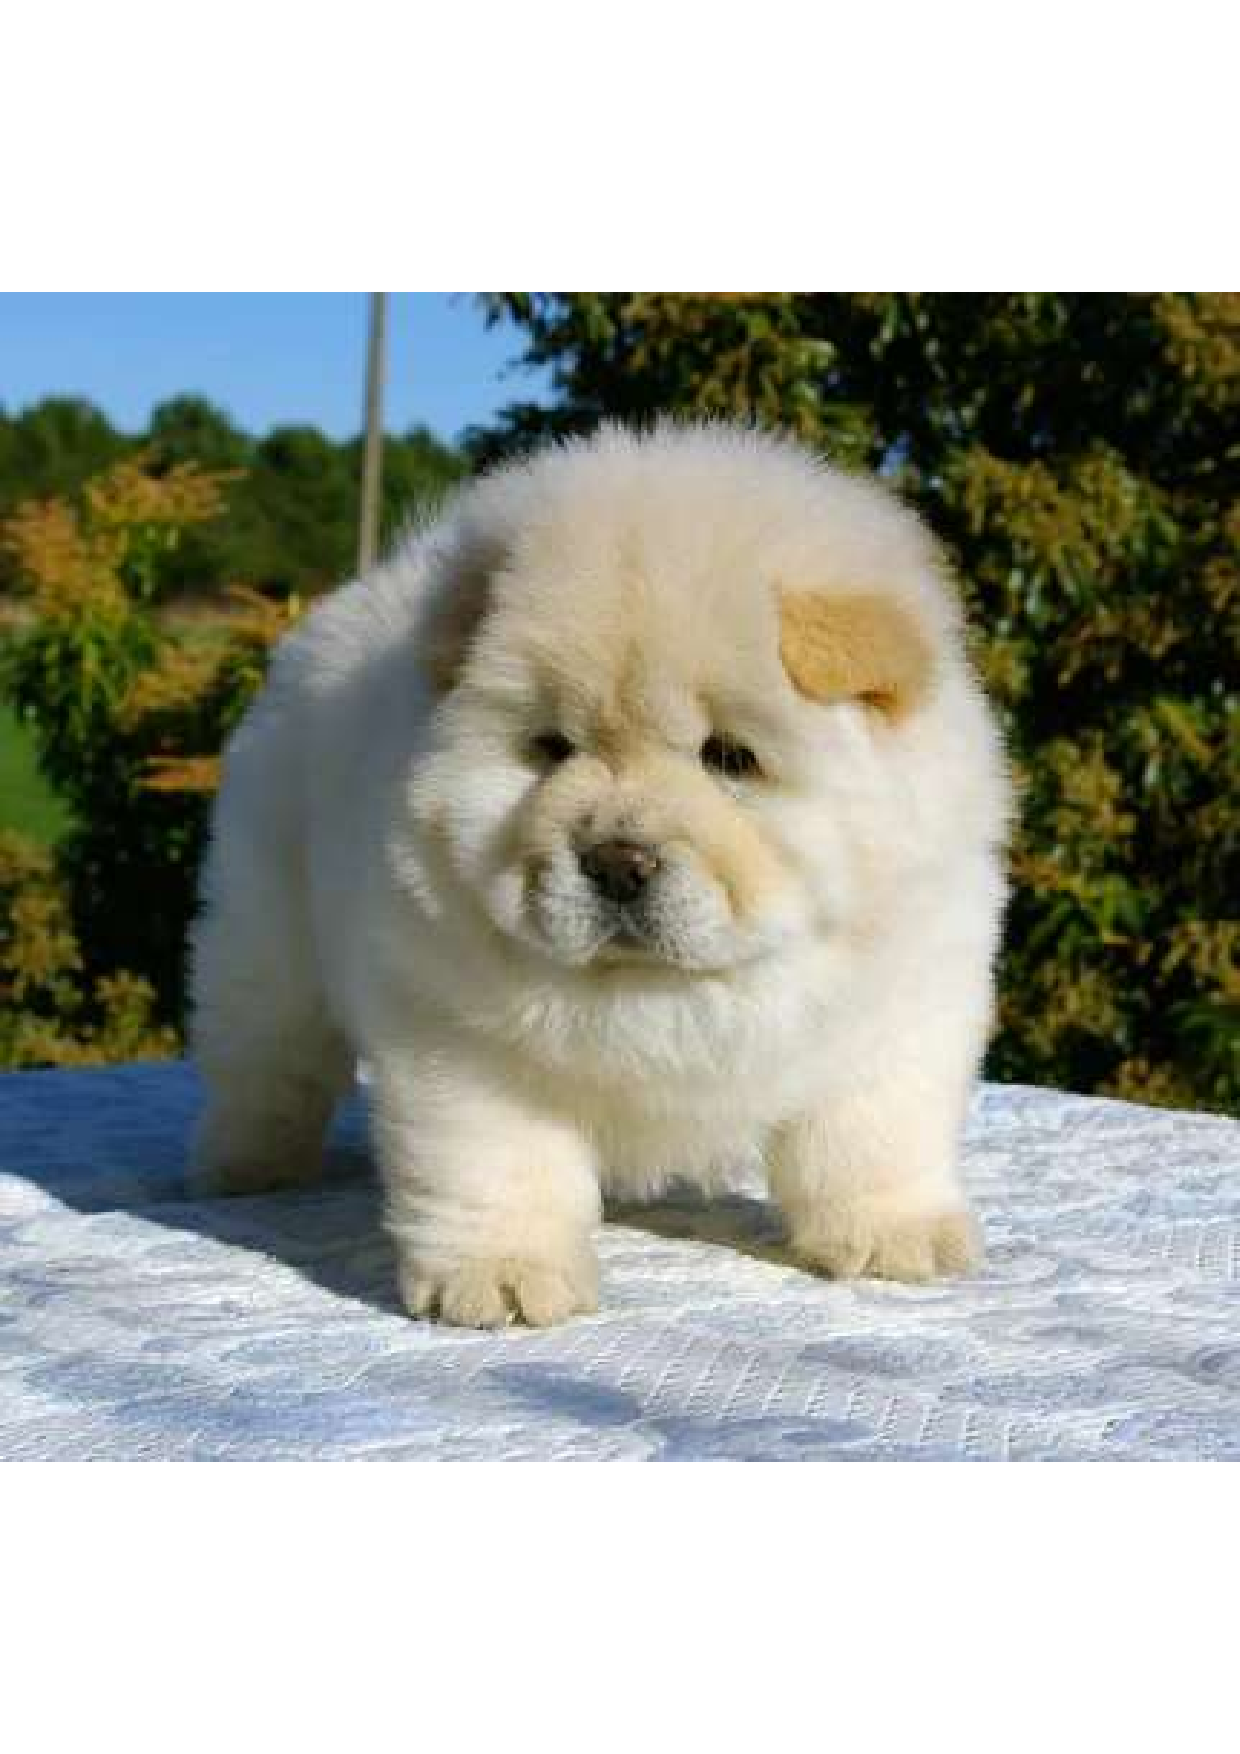
\includegraphics[height=7cm]{chowchow.pdf}\\
        \caption{{\emph{La jolie image !!!}}}
        \label{fig1}
    \end{center}
\end{figure}


\subsection{partie Maths}
Dans ce qui suit $E$ désigne un $K$ espace vectoriels 
\begin{theorem}
Soit $u \in \mathcal{L}(E)$. L'endomorphisme $u$ est symétrique si, et seulement si,
il existe une base orthonormale de $E$ composée de vecteurs propres de $u$. Dans ce cas, la matrice de $u$ dans cette base est diagonale.
\end{theorem}
\end{document}